\chapter{
  Introduction
 }\label{ch_intro}

``Particle Physics'' is the branch of physics which deals with the fundamental
particles and the interactions between them. Fundamental particles are the
subatomic particles currently known today which are not made of other particles.
There are two types of fundamental particles ``matter'' and ``interaction''
particles, matter particles are the fundamental constituent of matter and
the interactions between matter particle is governed by exchange of interaction particles.
\gls{SM} of particle physics is the theory that classifies these fundamental
particles and describes three out of four fundamental
interaction forces; electromagnetic, weak, and strong.

This chapter introduces briefly to the theory of \gls{SM}, Higgs mechanism,
spontaneous \gls{EWSB}, \gls{VBS}, and the motivation for the search of \gls{VBS}
in semileptonic decay channel ZV with leptonic decay of Z,
and hadronic decay of V (W/Z) to pair of quarks.

\section{
  Standard model
 }\label{ch_intro:standard-model}

In \gls{SM}, the matter particles are fermions and interaction particles are bosons.
Figure~\ref{fig:standard-model-details} lists
mass, electric charge, and spin of fermions and bosons in \gls{SM}.

Fermions obey Fermi-Dirac statistics and have half integer spin. They can be further
divided into leptons which have integral electric charge, and quarks which have
fractional electric charge. In addition to the electric charge, quarks also have
``color'' charge which comes from the theory of \gls{QCD}, and have a property called
``color confinement''. Color confinement is the reason quarks can not be isolated and
observed separately. The three generation in fermions only differs by the mass of
the particles. \gls{SM} also includes anti-fermions which are fermions with equal
magnitude and opposite sign.

Bosons obey Bose-Einstein statistics and have integral spin,
they are described by local gauge theory and are also called gauge boson.
Photons are the interaction particle of electromagnetic force, they are massless
and only interact with charged particles. Gluons are the mediator of strong force
between quarks, they are massless and also carries color charge. \Wplusminus{} and Z
are the vector bosons and mediator of weak force,
unlike photons and gluons they are massive. \Wplus{} and \Wminus{}
are antiparticles of each other, and Z is antiparticle of its own.

Introduction to \gls{SM}~\cite{Yang-Mill:1954} goes here.

\begin{figure}[!ht]
  \centering
  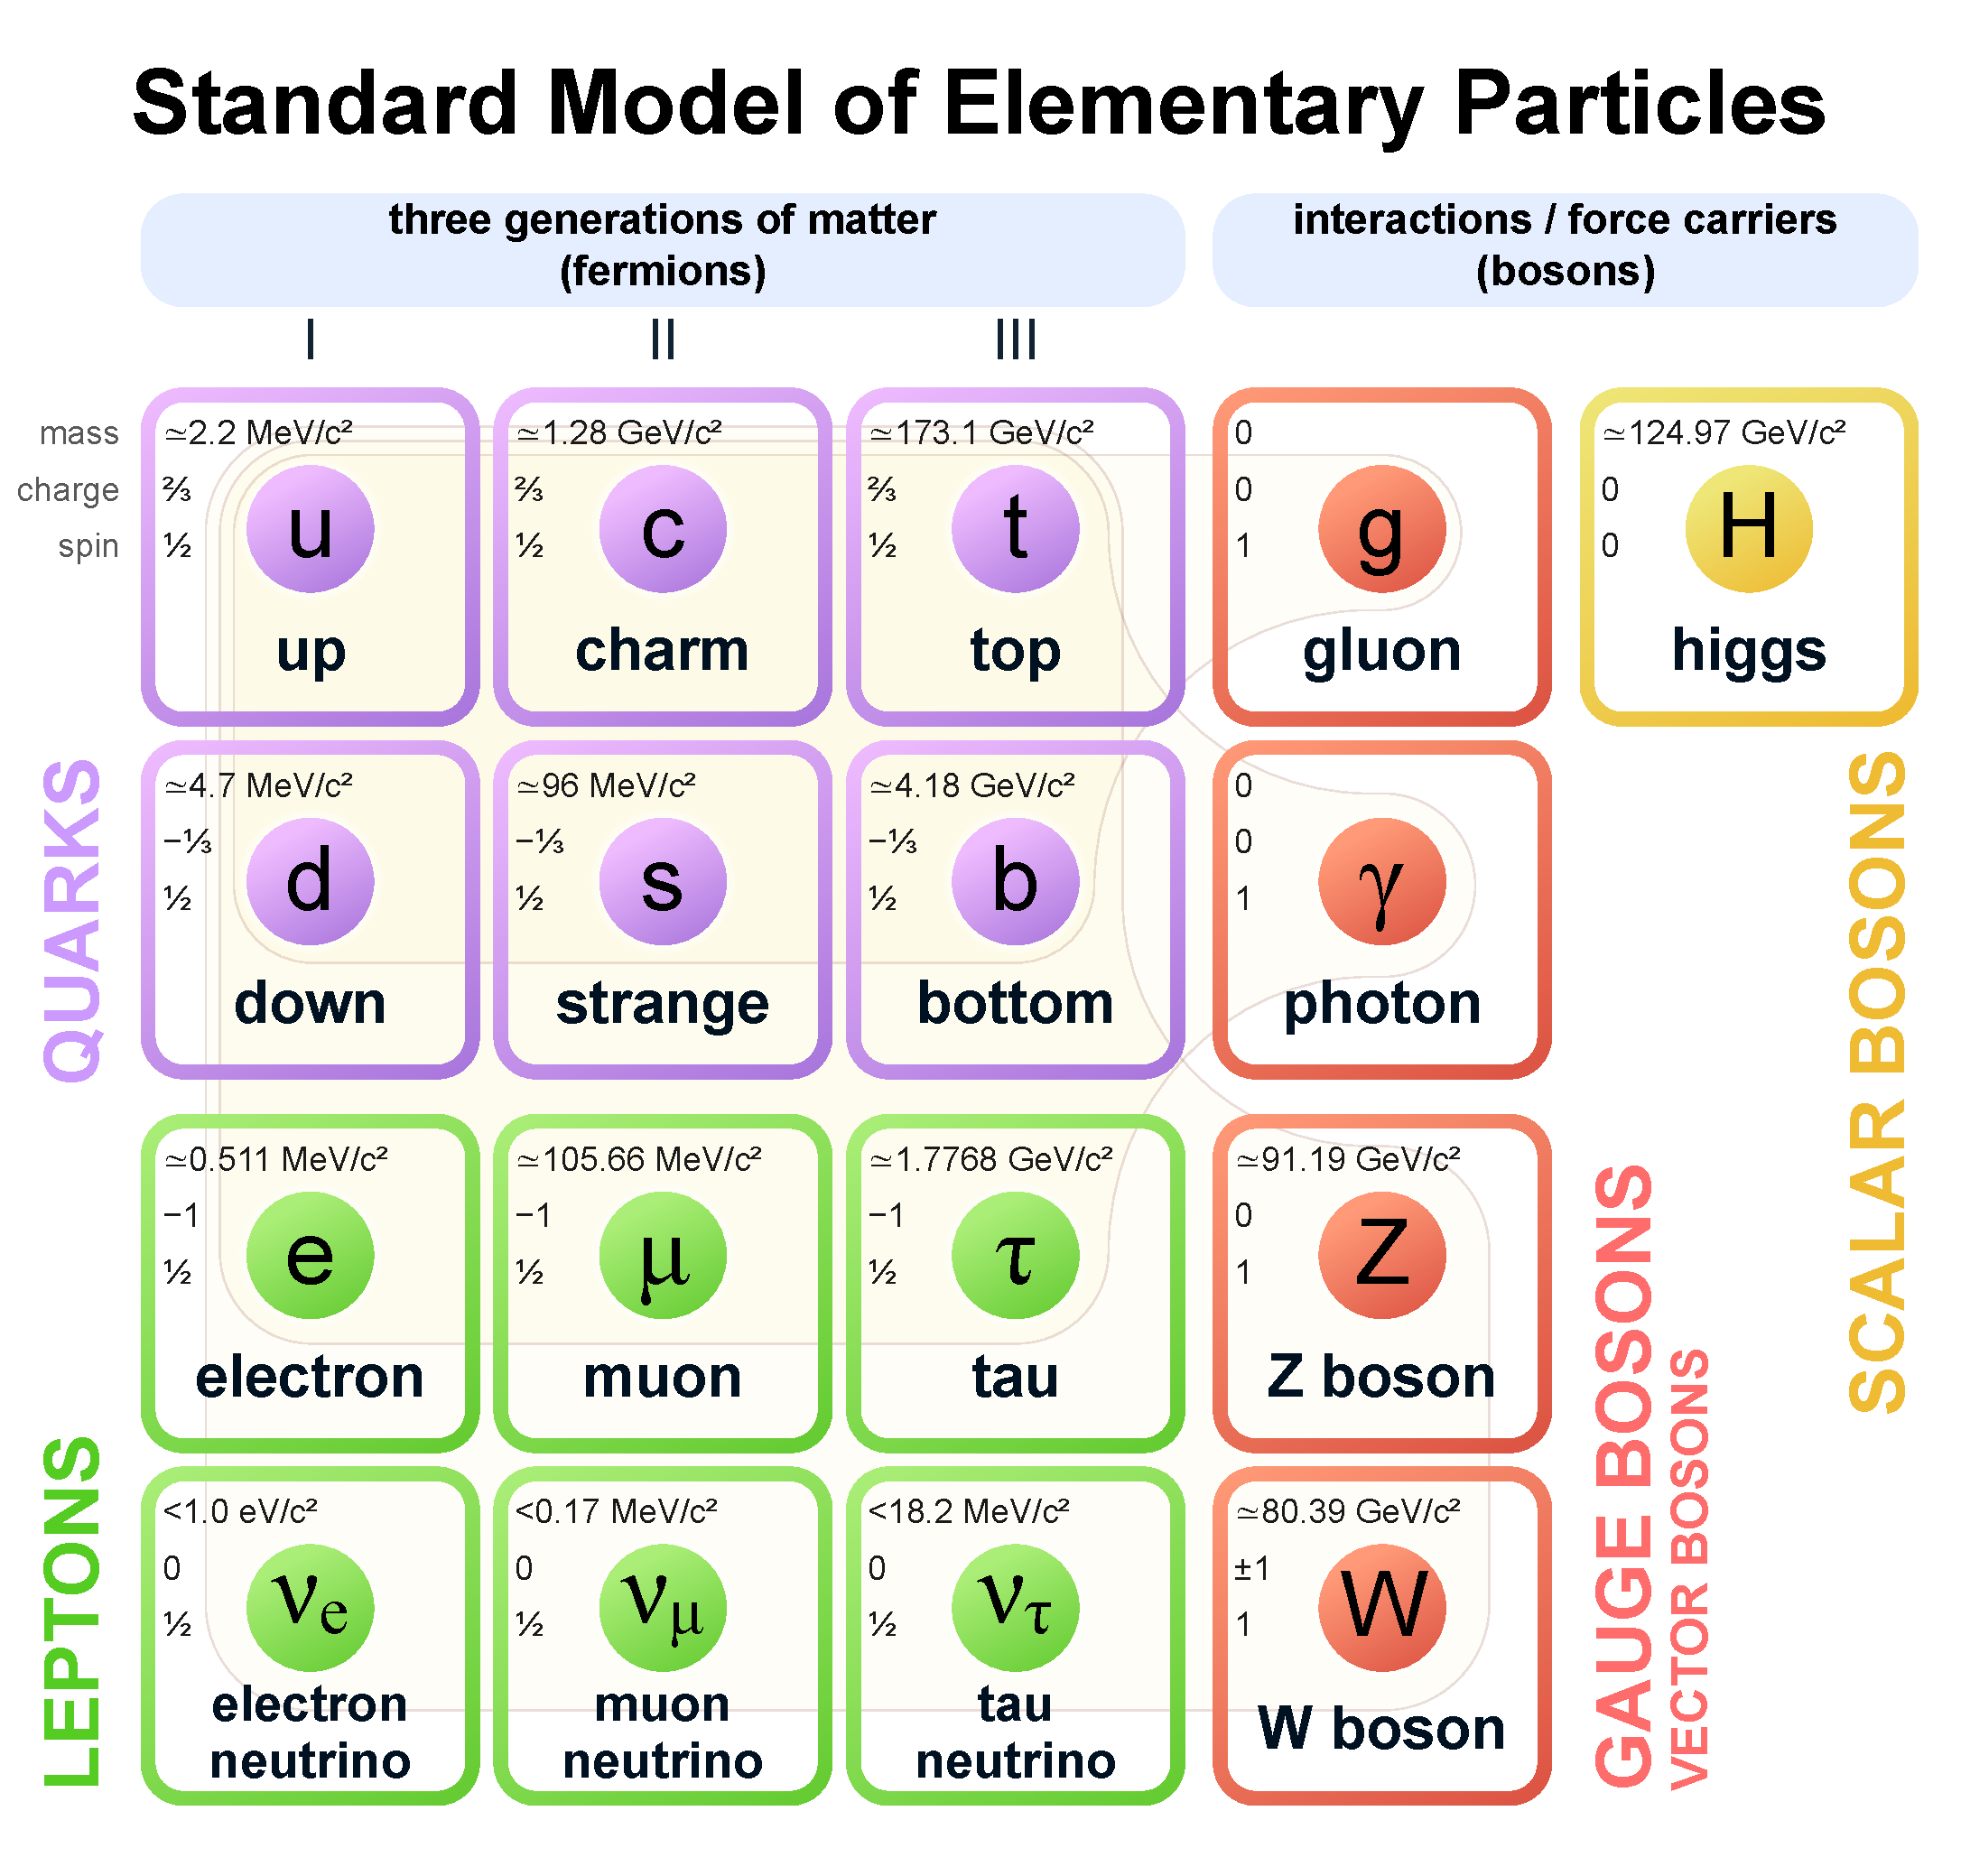
\includegraphics[width=0.8\textwidth]{figures/Standard_Model_of_Elementary_Particles.pdf}
  \caption[Standard model list of matter and interaction particles]%
  {Standard model list of matter and interaction particles~\cite{image-standard-model}}%
  \label{fig:standard-model-details}
\end{figure}

\begin{figure}[!ht]
  \centering
  \begin{minipage}{0.45\textwidth}
    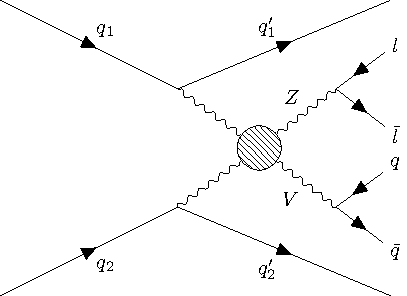
\includegraphics[width=\textwidth]{figures/feyn_vbs_0.pdf}
    \vspace{5pt}
  \end{minipage}
  \begin{minipage}{0.23\textwidth}
    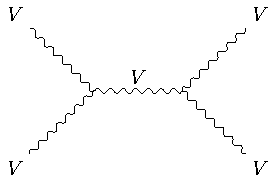
\includegraphics[width=\textwidth]{figures/feyn_vbs_2.pdf}
  \end{minipage}%
  \begin{minipage}{0.18\textwidth}
    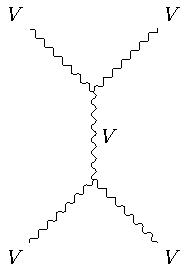
\includegraphics[width=\textwidth]{figures/feyn_vbs_4.pdf}
  \end{minipage}%
  \begin{minipage}{0.23\textwidth}
    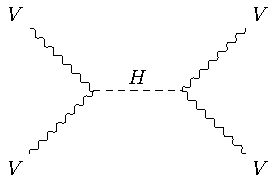
\includegraphics[width=\textwidth]{figures/feyn_vbs_3.pdf}
  \end{minipage}%
  \begin{minipage}{0.18\textwidth}
    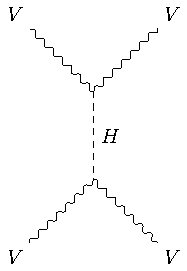
\includegraphics[width=\textwidth]{figures/feyn_vbs_5.pdf}
  \end{minipage}%
  \begin{minipage}{0.16\textwidth}
    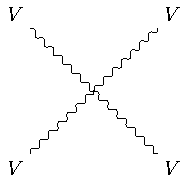
\includegraphics[width=\textwidth]{figures/feyn_vbs_1.pdf}
  \end{minipage}
\end{figure}

\section{Higgs Mechanism}

About Higgs Mechanism

\section{Vector Boson Scattering}

About fermions